\chapter{Bit manipulation}

All data in computer programs is internally stored as bits,
i.e., as numbers 0 and 1.
This chapter discusses the bit representation
of integers, and shows examples
of how to use bit operations.
It turns out that there are many uses for
bit manipulation in algorithm programming.

\section{Bit representation}

\index{bit representation}

In programming, an $n$ bit integer is internally
stored as a binary number that consists of $n$ bits.
For example, the C++ type \texttt{int} is
a 32-bit type, which means that every \texttt{int}
number consists of 32 bits.

Here is the bit representation of
the \texttt{int} number 43: 
\[00000000000000000000000000101011\]
The bits in the representation are indexed from right to left.
To convert a bit representation $b_k \cdots b_2 b_1 b_0$ into a number,
we can use the formula
\[b_k 2^k + \ldots + b_2 2^2 + b_1 2^1 + b_0 2^0.\]
For example,
\[1 \cdot 2^5 + 1 \cdot 2^3 + 1 \cdot 2^1 + 1 \cdot 2^0 = 43.\]

The bit representation of a number is either
\key{signed} or \key{unsigned}.
Usually a signed representation is used,
which means that both negative and positive
numbers can be represented.
A signed variable of $n$ bits can contain any
integer between $-2^{n-1}$ and $2^{n-1}-1$.
For example, the \texttt{int} type in C++ is
a signed type, so an \texttt{int} variable can contain any
integer between $-2^{31}$ and $2^{31}-1$.

The first bit in a signed representation
is the sign of the number (0 for nonnegative numbers
and 1 for negative numbers), and
the remaining $n-1$ bits contain the magnitude of the number.
\key{Two's complement} is used, which means that the
opposite number of a number is calculated by first
inverting all the bits in the number,
and then increasing the number by one.

For example, the bit representation of
the \texttt{int} number $-43$ is
\[11111111111111111111111111010101.\]

In an unsigned representation, only nonnegative
numbers can be used, but the upper bound for the values is larger.
An unsigned variable of $n$ bits can contain any
integer between $0$ and $2^n-1$.
For example, in C++, an \texttt{unsigned int} variable
can contain any integer between $0$ and $2^{32}-1$.

There is a connection between the
representations:
a signed number $-x$ equals an unsigned number $2^n-x$.
For example, the following code shows that
the signed number $x=-43$ equals the unsigned
number $y=2^{32}-43$:
\begin{lstlisting}
int x = -43;
unsigned int y = x;
cout << x << "\n"; // -43
cout << y << "\n"; // 4294967253
\end{lstlisting}

If a number is larger than the upper bound
of the bit representation, the number will overflow.
In a signed representation,
the next number after $2^{n-1}-1$ is $-2^{n-1}$,
and in an unsigned representation,
the next number after $2^{n-1}$ is $0$.
For example, consider the following code:
\begin{lstlisting}
int x = 2147483647
cout << x << "\n"; // 2147483647
x++;
cout << x << "\n"; // -2147483648
\end{lstlisting}

Initially, the value of $x$ is $2^{31}-1$.
This is the largest value that can be stored
in an \texttt{int} variable,
so the next number after $2^{31}-1$ is $-2^{31}$.


\section{Bit operations}

\newcommand\XOR{\mathbin{\char`\^}}

\subsubsection{And operation}

\index{and operation}

The \key{and} operation $x$ \& $y$ produces a number
that has one bits in positions where both
$x$ and $y$ have one bits.
For example, $22$ \& $26$ = 18, because

\begin{center}
\begin{tabular}{rrr}
& 10110 & (22)\\
\& & 11010 & (26) \\
\hline
 = & 10010 & (18) \\
\end{tabular}
\end{center}

Using the and operation, we can check if a number
$x$ is even because
$x$ \& $1$ = 0 if $x$ is even, and
$x$ \& $1$ = 1 if $x$ is odd.
More generally, $x$ is divisible by $2^k$
exactly when $x$ \& $(2^k-1)$ = 0.

\subsubsection{Or operation}

\index{or operation}

The \key{or} operation $x$ | $y$ produces a number
that has one bits in positions where at least one
of $x$ and $y$ have one bits.
For example, $22$ | $26$ = 30, because

\begin{center}
\begin{tabular}{rrr}
& 10110 & (22)\\
| & 11010 & (26) \\
\hline
 = & 11110 & (30) \\
\end{tabular}
\end{center}

\subsubsection{Xor operation}

\index{xor operation}

The \key{xor} operation $x$ $\XOR$ $y$ produces a number
that has one bits in positions where exactly one
of $x$ and $y$ have one bits.
For example, $22$ $\XOR$ $26$ = 12, because

\begin{center}
\begin{tabular}{rrr}
& 10110 & (22)\\
$\XOR$ & 11010 & (26) \\
\hline
 = & 01100 & (12) \\
\end{tabular}
\end{center}

\subsubsection{Not operation}

\index{not operation}

The \key{not} operation \textasciitilde$x$
produces a number where all the bits of $x$
have been inverted.
The formula \textasciitilde$x = -x-1$ holds,
for example, \textasciitilde$29 = -30$.

The result of the not operation at the bit level
depends on the length of the bit representation,
because the operation inverts all bits.
For example, if the numbers are 32-bit
\texttt{int} numbers, the result is as follows:

\begin{center}
\begin{tabular}{rrrr}
$x$ & = & 29 &   00000000000000000000000000011101 \\
\textasciitilde$x$ & = & $-30$ & 11111111111111111111111111100010 \\
\end{tabular}
\end{center}

\subsubsection{Bit shifts}

\index{bit shift}

The left bit shift $x < < k$ appends $k$
zero bits to the number,
and the right bit shift $x > > k$
removes the $k$ last bits from the number.
For example, $14 < < 2 = 56$,
because $14$ and $56$ correspond to 1110 and 111000.
Similarly, $49 > > 3 = 6$,
because $49$ and $6$ correspond to 110001 and 110.

Note that $x < < k$
corresponds to multiplying $x$ by $2^k$,
and $x > > k$
corresponds to dividing $x$ by $2^k$
rounded down to an integer.

\subsubsection{Applications}

A number of the form $1 < < k$ has a one bit
in position $k$ and all other bits are zero,
so we can use such numbers to access single bits of numbers.
In particular, the $k$th bit of a number is one
exactly when $x$ \& $(1 < < k)$ is not zero.
The following code prints the bit representation
of an \texttt{int} number $x$:

\begin{lstlisting}
for (int i = 31; i >= 0; i--) {
    if (x&(1<<i)) cout << "1";
    else cout << "0";
}
\end{lstlisting}

It is also possible to modify single bits
of numbers using similar ideas.
For example, the formula $x$ | $(1 < < k)$
sets the $k$th bit of $x$ to one,
the formula
$x$ \& \textasciitilde $(1 < < k)$
sets the $k$th bit of $x$ to zero,
and the formula
$x$ $\XOR$ $(1 < < k)$
inverts the $k$th bit of $x$.

The formula $x$ \& $(x-1)$ sets the last
one bit of $x$ to zero,
and the formula $x$ \& $-x$ sets all the
one bits to zero, except for the last one bit.
The formula $x$ | $(x-1)$
inverts all the bits after the last one bit.
Also note that a positive number $x$ is
a power of two exactly when $x$ \& $(x-1) = 0$.

\subsubsection*{Additional functions}

The g++ compiler provides the following
functions for counting bits:

\begin{itemize}
\item
$\texttt{\_\_builtin\_clz}(x)$:
the number of zeros at the beginning of the number
\item
$\texttt{\_\_builtin\_ctz}(x)$:
the number of zeros at the end of the number
\item
$\texttt{\_\_builtin\_popcount}(x)$:
the number of ones in the number
\item
$\texttt{\_\_builtin\_parity}(x)$:
the parity (even or odd) of the number of ones
\end{itemize}
\begin{samepage}

The functions can be used as follows:
\begin{lstlisting}
int x = 5328; // 00000000000000000001010011010000
cout << __builtin_clz(x) << "\n"; // 19
cout << __builtin_ctz(x) << "\n"; // 4
cout << __builtin_popcount(x) << "\n"; // 5
cout << __builtin_parity(x) << "\n"; // 1
\end{lstlisting}
\end{samepage}

While the above functions only support \texttt{int} numbers,
there are also \texttt{long long} versions of
the functions available with the suffix \texttt{ll}.

\section{Representing sets}

Every subset of a set
$\{0,1,2,\ldots,n-1\}$
can be represented as an $n$ bit integer
whose one bits indicate which
elements belong to the subset.
This is an efficient way to represent sets,
because every element requires only one bit of memory,
and set operations can be implemented as bit operations.

For example, since \texttt{int} is a 32-bit type,
an \texttt{int} number can represent any subset
of the set $\{0,1,2,\ldots,31\}$.
The bit representation of the set $\{1,3,4,8\}$ is
\[00000000000000000000000100011010,\]
which corresponds to the number $2^8+2^4+2^3+2^1=282$.

\subsubsection{Set implementation}

The following code declares an \texttt{int}
variable $x$ that can contain
a subset of $\{0,1,2,\ldots,31\}$.
After this, the code adds the elements 1, 3, 4 and 8
to the set and prints the size of the set.
\begin{lstlisting}
int x = 0;
x |= (1<<1);
x |= (1<<3);
x |= (1<<4);
x |= (1<<8);
cout << __builtin_popcount(x) << "\n"; // 4
\end{lstlisting}
Then, the following code prints all
elements that belong to the set:
\begin{lstlisting}
for (int i = 0; i < 32; i++) {
    if (x&(1<<i)) cout << i << " ";
}
// output: 1 3 4 8
\end{lstlisting}

\subsubsection{Set operations}

Set operations can be implemented as follows as bit operations:

\begin{center}
\begin{tabular}{lll}
& set syntax & bit syntax \\
\hline
intersection & $a \cap b$ & $a$ \& $b$ \\
union & $a \cup b$ & $a$ | $b$ \\
complement & $\bar a$ & \textasciitilde$a$ \\
difference & $a \setminus b$ & $a$ \& (\textasciitilde$b$) \\
\end{tabular}
\end{center}

For example, the following code first constructs
the sets $x=\{1,3,4,8\}$ and $y=\{3,6,8,9\}$,
and then constructs the set $z = x \cup y = \{1,3,4,6,8,9\}$:

\begin{lstlisting}
int x = (1<<1)+(1<<3)+(1<<4)+(1<<8);
int y = (1<<3)+(1<<6)+(1<<8)+(1<<9);
int z = x|y;
cout << __builtin_popcount(z) << "\n"; // 6
\end{lstlisting}

\subsubsection{Iterating through subsets}

The following code goes through
the subsets of $\{0,1,\ldots,n-1\}$:

\begin{lstlisting}
for (int b = 0; b < (1<<n); b++) {
    // process subset b
}
\end{lstlisting}
The following code goes through
the subsets with exactly $k$ elements:
\begin{lstlisting}
for (int b = 0; b < (1<<n); b++) {
    if (__builtin_popcount(b) == k) {
        // process subset b
    }
}
\end{lstlisting}
The following code goes through the subsets
of a set $x$:
\begin{lstlisting}
int b = 0;
do {
    // process subset b
} while (b=(b-x)&x);
\end{lstlisting}

\section{Bit optimizations}

It is often possible to optimize algorithms
using bit operations.
Such optimizations do not change the
time complexity of the algorithm,
but they may have a large impact
on the actual running time of the code.
In this section we discuss two examples
of such situations.

\subsubsection{Hamming distances}

\index{Hamming distance}
The \key{Hamming distance}
$\texttt{hamming}(a,b)$ between two
equal-length bit strings $a$ and $b$ is
the number of positions where the strings differ.
For example, $\texttt{hamming}(01101,11001)=2$.

Consider the following problem: Given
a list of $n$ bit strings, each of length $k$,
calculate the minimum Hamming distance
between two strings in the list.
For example, the answer for $[00111,01101,11110]$,
is 2, because
\begin{itemize}[noitemsep]
\item $\texttt{hamming}(00111,01101)=2$,
\item $\texttt{hamming}(00111,11110)=3$, and
\item $\texttt{hamming}(01101,11110)=3$.
\end{itemize}

A straightforward way to solve the problem is
to go through all pairs of string and calculate
their Hamming distances,
which yields an $O(n^2 k)$ time algorithm.
The following function calculates
the Hamming distance between two strings:
\begin{lstlisting}
int hamming(string a, string b) {
    int d = 0;
    for (int i = 0; i < k; i++) {
        if (a[i] != b[i]) d++;
    }
    return d;
}
\end{lstlisting}

However, if $k$ is small, we can optimize the code
by storing the bit strings as integers and
calculating the Hamming distances using bit operations.
In particular, if $k \le 32$, we can just store
the strings as \texttt{int} values and use the
following function to calculate distances:
\begin{lstlisting}
int hamming(int a, int b) {
    return __builtin_popcount(a^b);
}
\end{lstlisting}
In the above function, the xor operation constructs
a bit string that has one bits in positions
where $a$ and $b$ differ.
Then, the number of bits is calculated using
the \texttt{\_\_builtin\_popcount} function.

To compare the implementations, we generated
a list of 10000 random bit strings of length 30.
Using the first approach, the search took
13.5 seconds, and after the bit optimization,
it only took 0.5 seconds.
Thus, the bit optimized code was almost
30 times faster than the original code.

\subsubsection{Counting subgrids}

As another example, consider the
following problem:
Given an $n \times n$ grid whose
each square is either black or white,
calculate the number of subgrids
whose all corners are black.
For example, the grid
\begin{center}
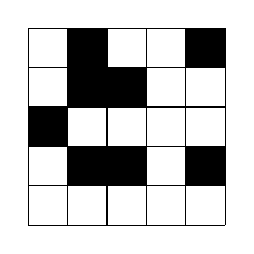
\begin{tikzpicture}[scale=0.5]
\fill[black] (1,1) rectangle (2,2);
\fill[black] (1,4) rectangle (2,5);
\fill[black] (4,1) rectangle (5,2);
\fill[black] (4,4) rectangle (5,5);
\fill[black] (1,3) rectangle (2,4);
\fill[black] (2,3) rectangle (3,4);
\fill[black] (2,1) rectangle (3,2);
\fill[black] (0,2) rectangle (1,3);
\draw (0,0) grid (5,5);
\end{tikzpicture}
\end{center}
contains two such subgrids:
\begin{center}
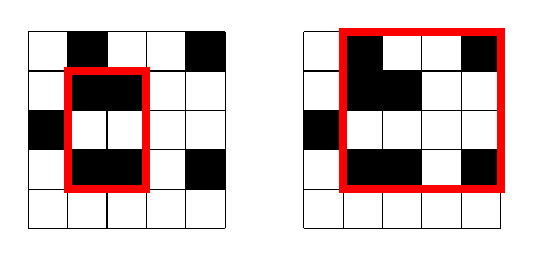
\begin{tikzpicture}[scale=0.5]
\fill[black] (1,1) rectangle (2,2);
\fill[black] (1,4) rectangle (2,5);
\fill[black] (4,1) rectangle (5,2);
\fill[black] (4,4) rectangle (5,5);
\fill[black] (1,3) rectangle (2,4);
\fill[black] (2,3) rectangle (3,4);
\fill[black] (2,1) rectangle (3,2);
\fill[black] (0,2) rectangle (1,3);
\draw (0,0) grid (5,5);

\fill[black] (7+1,1) rectangle (7+2,2);
\fill[black] (7+1,4) rectangle (7+2,5);
\fill[black] (7+4,1) rectangle (7+5,2);
\fill[black] (7+4,4) rectangle (7+5,5);
\fill[black] (7+1,3) rectangle (7+2,4);
\fill[black] (7+2,3) rectangle (7+3,4);
\fill[black] (7+2,1) rectangle (7+3,2);
\fill[black] (7+0,2) rectangle (7+1,3);
\draw (7+0,0) grid (7+5,5);

\draw[color=red,line width=1mm] (1,1) rectangle (3,4);
\draw[color=red,line width=1mm] (7+1,1) rectangle (7+5,5);
\end{tikzpicture}
\end{center}

There is an $O(n^3)$ time algorithm for solving the problem:
go through all $O(n^2)$ pairs of rows and for each pair
calculate the number of columns that contain a black
square in both rows in $O(n)$ time.
Then, if there are $c$ such columns for a fixed row pair,
they account for $c(c-1)/2$ subgrids with black corners.

To optimize this algorithm, we divide the grid into blocks
of columns such that each block consists of $N$
consecutive columns. Then, each row is stored as
a list of $N$-bit numbers that describe the colors
of the squares.
Using this representation,
we can process $N$ columns at the same time
using bit operations, and the resulting algorithm
works in $O(n^3/N)$ time.

We generated a random grid of size $2500 \times 2500$
and compared the original and bit-optimized implementation.
While the original code took $29.6$ seconds,
the bit-optimized version only took $3.1$ seconds
with $N=32$ (\texttt{int} numbers) and $1.7$ seconds
with $N=64$ (\texttt{long long} numbers).

\section{Dynamic programming}

\subsubsection{From permutations to subsets}

Using dynamic programming, it is often possible
to change an iteration over permutations into
an iteration over subsets, so that
the dynamic programming state
contains a subset of a set and possibly
some additional information\footnote{This technique was introduced in 1962
by M. Held and R. M. Karp \cite{hel62}.}.

The benefit of this is that
$n!$, the number of permutations of an $n$ element set,
is much larger than $2^n$, the number of subsets
of the same set.
For example, if $n=20$, then
$n! \approx 2.4 \cdot 10^{18}$ and $2^n \approx 10^6$.
Hence, for certain values of $n$,
we can efficiently go through subsets but not through permutations.

As an example, consider the following problem:
There is an elevator with maximum weight $x$,
and $n$ people with known weights
who want to get from the ground floor
to the top floor.
What is the minimum number of rides needed
if the people enter the elevator in an optimal order?

For example, suppose that $x=10$, $n=5$
and the weights are as follows:
\begin{center}
\begin{tabular}{ll}
person & weight \\
\hline
$A$ & 2 \\
$B$ & 3 \\
$C$ & 3 \\
$D$ & 5 \\
$E$ & 6 \\
\end{tabular}
\end{center}
In this case, the minimum number of rides is 2.
One optimal order is $\{A,C,D,B,E\}$,
which partitions the people into two rides:
first $\{A,C,D\}$ (total weight 10),
and then $\{B,E\}$ (total weight 9).

The problem can be easily solved in $O(n! n)$ time
by testing all possible permutations of $n$ people.
However, we can use dynamic programming to get
a more efficient $O(2^n n)$ time algorithm.
The idea is to calculate for each subset of people
two values: the minimum number of rides needed and
the minimum weight of people who ride in the last group.

Let $\texttt{rides}(X)$ denote the minimum number
of rides and $\texttt{weight}(X)$ denote the minimum
weight of the last group, where $X$ is a subset
of people. For example,
\[ \texttt{rides}(\{B,D,E\})=2 \hspace{10px} \textrm{and}
\hspace{10px} \texttt{weight}(\{B,D,E\})=5,\]
because the optimal rides are $\{B,E\}$ and $\{D\}$,
and the second ride has weight 5.
Of course, our final goal is to calculate the value
of $\texttt{rides}(\{A,B,C,D,E\})$ that is the solution
to the problem.

It turns out that we can calculate the values
of the functions recursively and then apply
dynamic programming.
The idea is to go through all people
that belong to $X$ and optimally
choose the last person who enters the elevator.
For example, if $X=\{B,D,E\}$,
one of $B$, $D$ and $E$ is the last person
who enters the elevator.
Each such choice yields a subproblem
for a smaller subset of people.

\subsubsection{Counting subsets}

Our last problem in this chapter is as follows:
We are given a collection $C$ that consists of $m$ sets,
and our task is to determine for each set
the number of sets in $C$ that are its subsets.
For example, consider the following collection:
\[C = \{\{0\}, \{0,2\}, \{1,4\}, \{0,1,4\}, \{1,4,5\}\}\]
For any set $x$ in $C$,
let $f(x)$ denote the number of sets (including $x$) in $C$
that are subsets of $x$.
For example, $f(\{0,1,4\})=3$, because the
sets $\{0\}$, $\{1,4\}$ and $\{0,1,4\}$ are
subsets of $\{0,1,4\}$.
Using this notation, our task is to calculate the value of $f(x)$
for every set $x$ in the collection.

We will assume that each set is
a subset of $\{0,1,\ldots,n-1\}$.
Thus, the collection can contain at most
$2^n$ sets.
A straightforward way to solve the problem
is to go through all pairs of sets in the collection.
However, a more efficient solution is possible
using dynamic programming.

Let $c(x,k)$ denote the number of sets in
$C$ that equal a set $x$
if we are allowed to remove any subset of
$\{0,1,\ldots,k\}$ from $x$.
For example, in the above collection,
$c(\{0,1,4\},1)=2$,
where the corresponding sets are
$\{1,4\}$ and $\{0,1,4\}$.

It turns out that we can calculate all
values of $c(x,k)$ in $O(2^n n)$ time.
This solves our problem, because
\[f(x)=c(x,n-1).\]

The base cases for the function are:
\begin{equation*}
    c(x,-1) = \begin{cases}
               0 & \textrm{if $x \notin C$}\\
               1 & \textrm{if $x \in C$}\\
           \end{cases}
\end{equation*}
For larger values of $k$, the following recursion holds:
\begin{equation*}
    c(x,k) = \begin{cases}
               c(x,k-1)          & \textrm{if $k \notin x$}\\
               c(x,k-1)+c(x \setminus \{k\},k-1)    & \textrm{if $k \in x$}\\
           \end{cases}
\end{equation*}

We can conveniently implement the algorithm by representing
the sets using bits.
Assume that there is an array
\begin{lstlisting}
int d[1<<n];
\end{lstlisting}
that is initialized so that $d[x]=1$ if $x$ belongs to $C$
and otherwise $d[x]=0$.
We can now implement the algorithm as follows:

\begin{lstlisting}
for (int k = 0; k < n; k++) {
    for (int b = 0; b < (1<<n); b++) {
        if (b&(1<<k)) d[b] += d[b^(1<<k)];
    }
}
\end{lstlisting}
The above code is based on the recursive definition
of $c$. As a special trick, the code only uses
the array $d$ to calculate all values of the function.
Finally, for each set $x$ in $C$, $f(x)=d[x]$.

